\chapter{Background}

This chapter provides the background information necessary to understand this report. It covers topics such as the development of large software systems, types of software systems, their maintenance, analysis, and other related concepts.

\section{The Software Lifecycle: From Idea to Execution}

Developing a large software system is a complex and crucial process that requires careful planning and execution. A large scale software system involves many interconnected components, all of which must adhere to essential software development principles. The goal is not just to write code but to build a system that is reliable, maintainable, scalable, and efficient. Ensuring the system is free of bugs and capable of adapting to future needs is as important as the initial development itself. By following these key paradigms, developers can create software that meets high standards of quality and performance.

\begin{figure}[H]
    \centering
    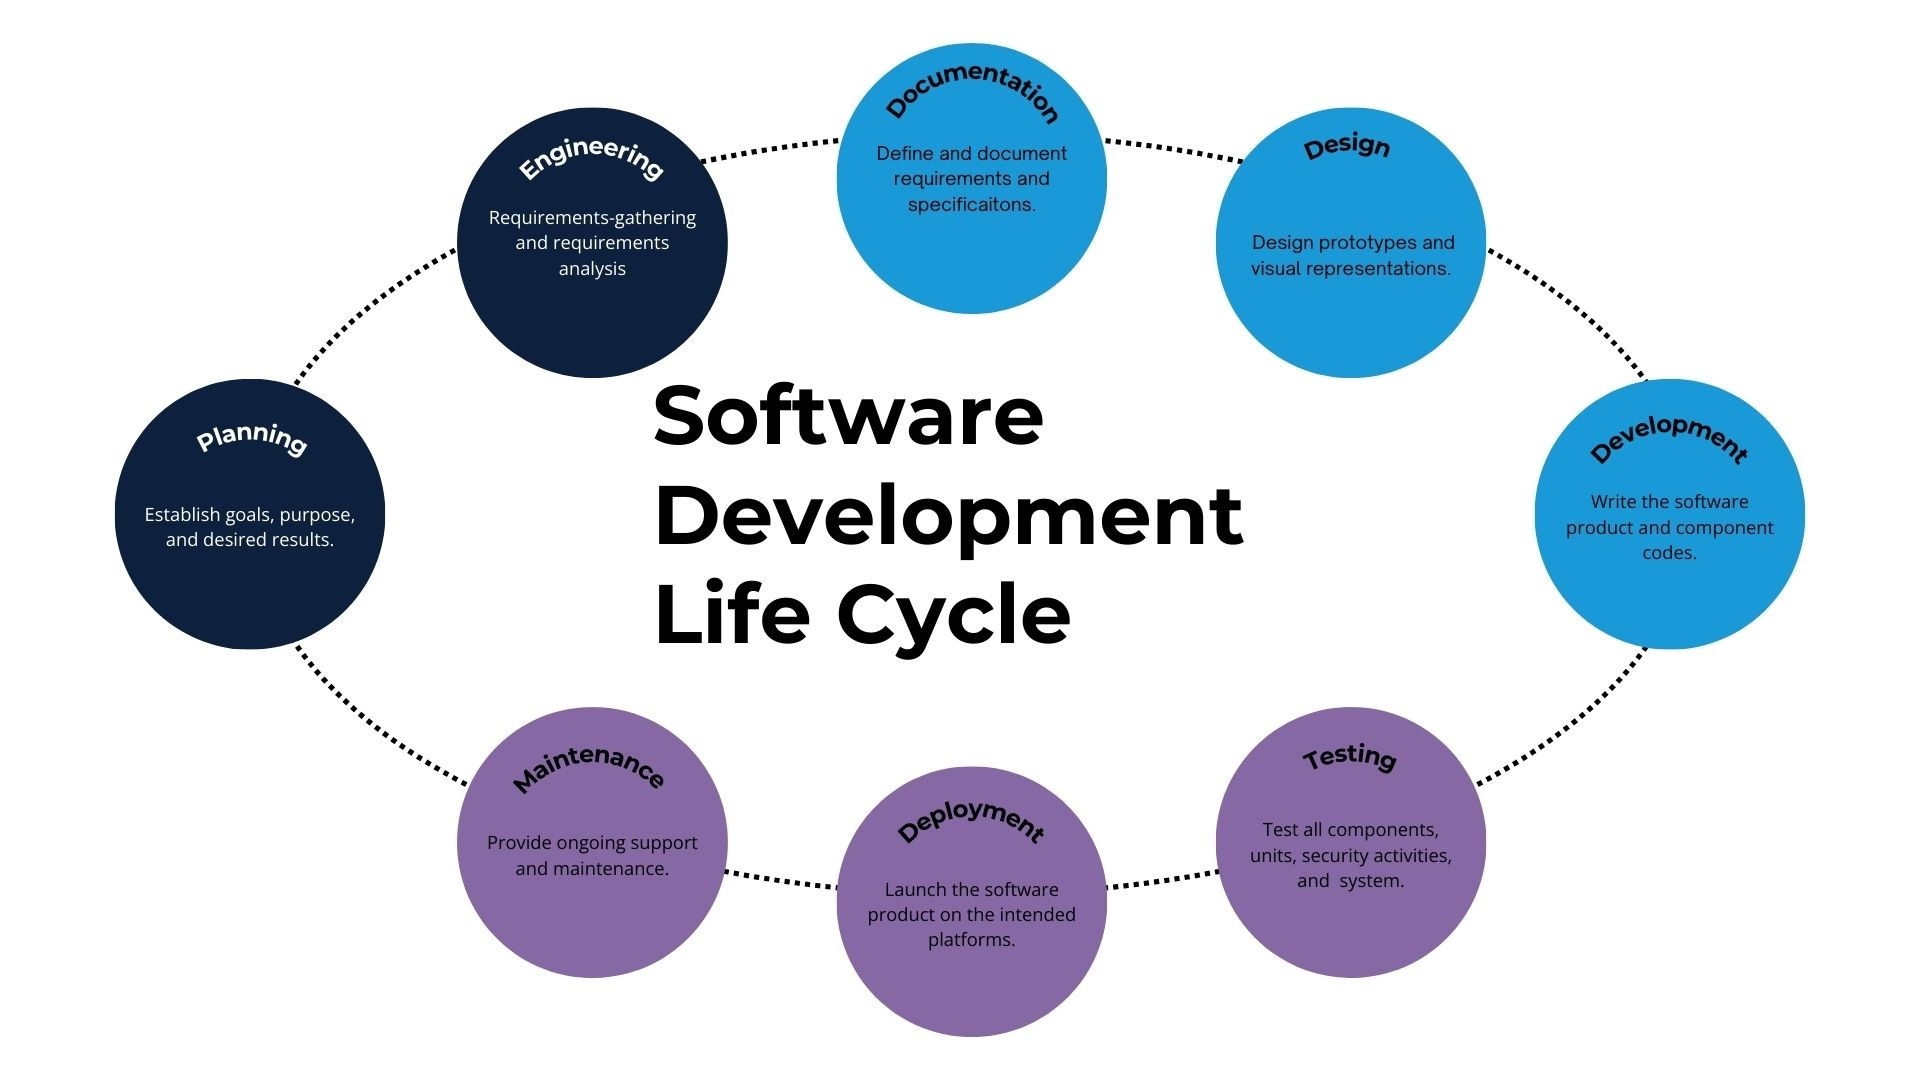
\includegraphics[width=1\textwidth]{figures/software_development.png}
    \caption{Software Development Life cycle (adapted from~\citep{sire_sdlc_2024})}
	\label{fig_background_sd}
\end{figure}

Each phase of the software development process adds an important contribution to the overall project. For example, in the planning and engineering phase, the team works closely with stakeholders to determine the functional and non-functional requirements of the project. This collaboration ensures that everyone involved understands the project's goals and technical needs. In the documentation phase, all the information gathered during planning and engineering is carefully recorded. This creates a detailed reference for the team, helping maintain consistency and clarity as the project progresses.

Following the Software Development Life Cycle (SDLC) provides several key benefits. It helps in identifying clear goals, ensures all stakeholders are on the same page, and allows for thorough testing at every stage. This structured approach produces high-quality software systems and maintains a smooth and understandable development flow. By sticking to the SDLC, teams can reduce risks, avoid confusion, and create software that meets user expectations.

Once the major development work is complete, the focus shifts towards software maintenance. Maintaining a large project becomes a significant task in itself. Updates, bug fixes, and adapting to new requirements or technologies are ongoing responsibilities. Without proper maintenance, even the best-designed systems can become outdated or difficult to use.

\section{Software Maintenance in Large Systems}

Since an already built large software system is quite complex, understanding this system requires certain strategies and tools. When a problem arises in complex software architectures, such as microservices or service-oriented architectures, resolving it often demands significant resources. These architectures consist of numerous interconnected components, and identifying the root cause of an issue can be challenging. The process may involve extensive debugging, analyzing logs, coordinating between multiple teams, and sometimes even re-evaluating design decisions. This can result in considerable time, effort, and cost being spent to restore functionality and ensure the system operates smoothly.~\citep{Folmer2005} discusses the usability issues in software systems post-development and highlights that they require significant architectural changes. In order to deal with such architectural changes, an understanding of the whole system is required, and if the system is large enough, major resources are spent fixing even minor issues.

~\citep{SeMaintainance2001} states that several surveys indicate that software maintenance consumes 60\% to 80\% of the total life cycle costs. Also, the maintenance costs are largely due to enhancement (often 75{-}80\%), rather than corrections. To address these challenges, there is a growing need for tools that can assist in resolving bugs and reducing maintenance overhead. Such tools should be capable of reverse engineering software systems to provide a clear and comprehensive view of the architecture. By highlighting the key components and their interactions, these tools make it easier for developers to understand the system, identify issues, and perform necessary tasks efficiently. This not only simplifies debugging but also enhances the overall maintainability of the software, ensuring smoother operation and reduced downtime.

\begin{figure}[H]
    \centering
    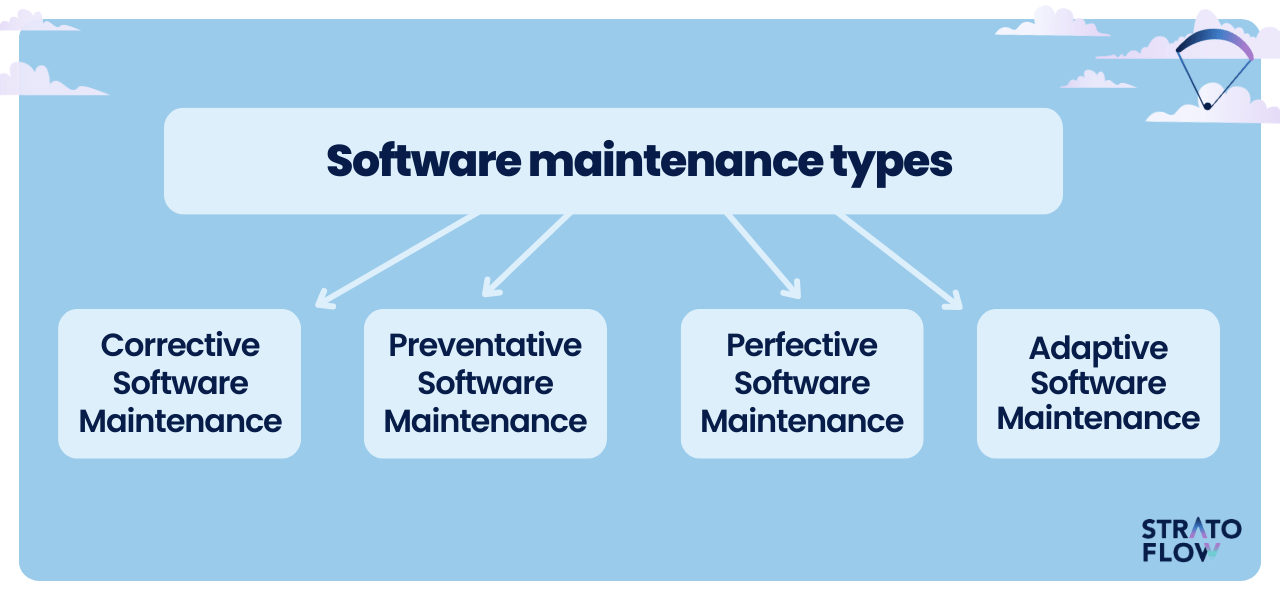
\includegraphics[width=0.9\textwidth]{figures/se_maintenance.png}
    \caption[Software Maintenance Types]{Software Maintenance Types (adapted from~\cite{stratoflow2025})}
	\label{fig_se_maintenance}
\end{figure}

\section{Software Architectures}
Software architecture is the fundamental structure of a software system.~\citep{sei_software_architecture} refers software architectures as the ``representation of the design decisions related to overall system structure and behavior. Architecture helps stakeholders understand and analyze how the system will achieve essential qualities such as modifiability, availability, and security''.

Each architecture has its own pros and cons. There are different types of software architectures adopted or sometimes introduced in order to solve certain issues. The most important ones that are necessary to be understood for this report are monolithic and microservices architectures.

\subsection{Monolithic Architecture}
Monolithic architecture is a traditional software development design paradigm where an application is built as a single, unified unit. All the components of the system are tightly coupled and dependent on each other. The monolithic architecture is simple, easier to design, develop and test and usually have easier deployment process as compared to some other architectures.

\subsection{Microservice Architecture}
Microservice architecture is a software design in which a system is built as a collection of small, independent, and loosely coupled services. Each service is designed to keep in mind the Single-responsibility principle and hence have a specific function, operates independently and communicates with other services typically using HTTP or messaging queues. Microservice architecture is easier to scale, flexible, autonomous and more resilient than other architectures, especially monolithic. 

\begin{figure}[H]
    \centering
    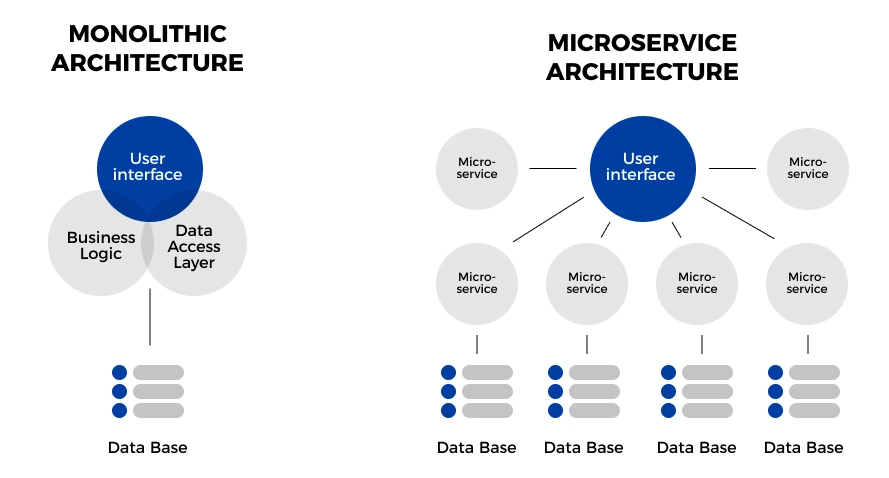
\includegraphics[width=0.9\textwidth]{figures/monolithic_microservices.png}
    \caption{Monolithic vs Microservices Architecture (adapted from~\cite{atlassian_microservices_vs_monolith})}
	\label{fig_background_monolithic_microservices}
\end{figure}

The figure~\ref{fig_background_monolithic_microservices} shows the difference between the monolithic and microservice architecture. In monolithic, all the components of the software system are combined in a single unit whereas in microservice architecture, the whole system is divided into smaller autonomous components. These individual components are easier to manage, scale, maintain and debug.

One of the key challenges in software development is understanding the system’s architecture after the major development process is completed or stabilized. Developing a software system often takes years of effort and significant resources. As a result, fully grasping its complexity can be difficult, especially for teams that were not involved in the original development.

To overcome this challenge, proper documentation, well-defined workflows, and effective knowledge transfer are essential. However, even with these measures, there are instances where critical system insights are required to diagnose issues efficiently. In such cases, improved documentation and deeper system analysis become necessary. This is why \textbf{reverse engineering} is often applied to existing or legacy systems to gain a clear understanding of their structure and functionality.

\section{Understanding Reverse Engineering}  
\citep{digitalai_reverse_engineering} states that 
\begin{tcolorbox}[colback=gray!10, colframe=gray!20]
	``The goal of reverse engineering is to reveal the logic, features, and functionalities embedded within the software.''
\end{tcolorbox}

An article by~\citep{twoFacesOfSRE} discusses that software reverse engineering can be achieved through several approaches:
\begin{itemize}
    \item \textbf{Observation-Based Analysis:} Involves studying the exchange of information within the software to infer its functionality and behavior.
    \item \textbf{Disassembly:} Utilizes a disassembler to interpret and analyze the program's raw machine code.
    \item \textbf{Decompilation:} Employs a decompiler to attempt reconstruction of the program’s source code in a high-level language, starting from machine code or bytecode.
\end{itemize}

\begin{figure}[H]
    \centering
    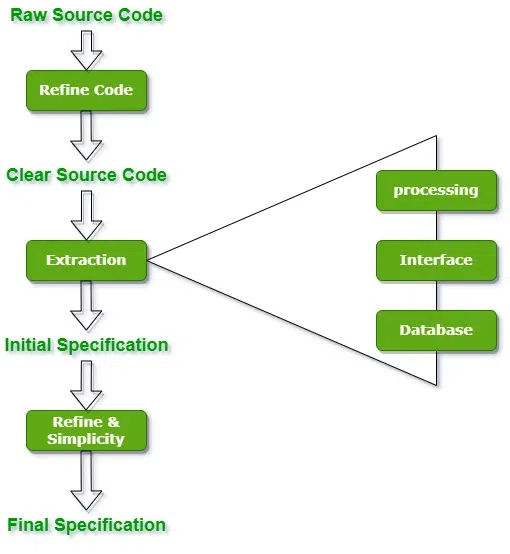
\includegraphics[width=0.75\textwidth]{figures/Reverse-Engineering.png}
    \caption{Reverse Engineering (adapted from~\cite{geeksforgeeks2024})}
	\label{fig_background_reverse_engineering}
\end{figure}

As shown in figure~\ref{fig_background_reverse_engineering}, source code is refined and analyzed to derive a final specification.

\begin{itemize}
    \item The process begins with the raw source code of a software application.
    \item The raw source code is refined to make it cleaner, more organized, and readable by removing unnecessary parts.
    \item The process of extraction identifies key elements of the system.
    \item An initial specification of the system is created, outlining the system's structure and behavior.
    \item The initial specification is then further refined to ensure simplicity and reducing complexity.
    \item The process concludes with a final specification, which is a clear description of the system's design, functionality, and architecture.
\end{itemize}


In the later chapters of this report, we will discuss a framework that uses static analysis of source code. This framework aids in reverse engineering by disassembling the system and generating valuable insights.
